\documentclass[conference]{IEEEtran}
\IEEEoverridecommandlockouts
% The preceding line is only needed to identify funding in the first footnote. If that is unneeded, please comment it out.
\usepackage{cite}
\usepackage{amsmath,amssymb,amsfonts}
\usepackage{algorithmic}
\usepackage{graphicx}
\usepackage{textcomp}
\usepackage{xcolor}

\def\BibTeX{{\rm B\kern-.05em{\sc i\kern-.025em b}\kern-.08em
    T\kern-.1667em\lower.7ex\hbox{E}\kern-.125emX}}
\begin{document}

\title{Augmented Reality in Education
}

\author{\IEEEauthorblockN{Tobias Wen Klingenberg}
\IEEEauthorblockA{\textit{School of Computation, Information and Technology} \\
\textit{Technische Universität München}\\
München, Deutschland \\
t.klingenberg@tum.de}
}
\maketitle

\begin{abstract}
Das folgende Paper befasst sich mit der Entwicklung, 
Anwendung und Analyse der Möglichkeiten von Augmented Reality 
in all seinen Formen im Hinblick auf Bildung in den verschiedensten Bildungsstufen und Formen
\end{abstract}

\section{Einleitung}
Augmented Reality (im Folgenden AR) ist eine Innovation, welche in den letzten
Jahren immer mehr Akzeptanz und tatsächliche Anwendung in unserem täglichen
Leben genießen konnte. Sie ist eine Technologie, welche es ermöglicht, digitale
Informationen mit der echten physischen Welt zu überlagern und somit die persönliche 
Sicht "erweitern". 

Dazu gibt es verschiedenste Innovationen, die dieses Konzept 
auf unterschiedlicher Weise ermöglichen. Durch diese Verschmelzung
der digitalen und realen Welt eröffnen sich vollkommen neue Anwendungsmöglichkeiten
, wie unter anderem interaktive Lernumgebungen, Unterstützung im medizinischen Bereich
oder Unterhaltungs- und Unterstützungsmedien. Im Folgenden wird vor allem auf die möglichen 
Anwendungen im Bildungsbereich eingegangen.


\section{Warum AR}

AR bietet sich vor allem aus mehreren Gründen für eine Anwendung in den verschiedensten
Bildungsmöglichkeiten an. Dazu gehört vor allem eine stärkere Gedächtnisleistung aufgrund von
visuellen und interaktiven Inhalten, sowie ein personalisiertes Lernen durch Anpassung 
auf individuell nötigen Bedürfnissen \cite{b1}. 

Eine hohe Motivation unter den Schüler:innen 
kann mit Ansätzen einer spielerischen Bildung ermöglicht werden. Vor allem interssant ist 
die mögliche kontextualisierte Lernerfahrung, indem theoretisches Wissen in simulierten 
Umgebungen angewedent werden kann \cite{b2}. TODO

\section{Entwicklung}
In den vergangen Jahren ließ sich eine immer höhrer Nachfrage für AR Technologien im Bildungsbereich
feststellen. Vor allem in der Forschung ist dieser Trend sichtbar, in der tatsächlichen Anwendung
Dies hat verschiedene Gründe. 

\section{AR-Tools und Plattformen}\label{AA}
Define abbreviations and acronyms the first time they are used in the text, 
even after they have been defined in the abstract. Abbreviations such as 
IEEE, SI, MKS, CGS, ac, dc, and rms do not have to be defined. Do not use 
abbreviations in the title or heads unless they are unavoidable.

\subsection{Software}
Blabla

\subsection{Hardware}
Number equations consecutively. To make your 
equations more compact, you may use the solidus (~/~), the exp function, or 
appropriate exponents. Italicize Roman symbols for quantities and variables, 
but not Greek symbols. Use a long dash rather than a hyphen for a minus 


\section{Anwendungen}
\textbf{The class file is designed for, but not limited to, six authors.} A 
minimum of one author is required for all conference articles. Author names 
should be listed starting from left to right and then moving down to the 
next line. This is the author sequence that will be used in future citations 
and by indexing services. Names should not be listed in columns nor group by 
affiliation. Please keep your affiliations as succinct as possible (for 
example, do not differentiate among departments of the same organization).

\subsection{Primär und Sekundär}
Headings, or heads, are organizational devices that guide the reader through 
your paper. There are two types: component heads and text heads.

Component heads identify the different components of your paper and are not 
topically subordinate to each other. Examples include Acknowledgments and 
References and, for these, the correct style to use is ``Heading 5''. Use 
``figure caption'' for your Figure captions, and ``table head'' for your 
table title. Run-in heads, such as ``Abstract'', will require you to apply a 
style (in this case, italic) in addition to the style provided by the drop 
down menu to differentiate the head from the text.

Text heads organize the topics on a relational, hierarchical basis. For 
example, the paper title is the primary text head because all subsequent 
material relates and elaborates on this one topic. If there are two or more 
sub-topics, the next level head (uppercase Roman numerals) should be used 
and, conversely, if there are not at least two sub-topics, then no subheads 
should be introduced.

\subsection{Hochschule}
Place figures and tables at the top and 
bottom of columns. Avoid placing them in the middle of columns. Large 
figures and tables may span across both columns. Figure captions should be 
below the figures; table heads should appear above the tables. Insert 
figures and tables after they are cited in the text. Use the abbreviation 
``Fig.~\ref{fig}'', even at the beginning of a sentence.

\begin{table}[htbp]
\caption{Table Type Styles}
\begin{center}
\begin{tabular}{|c|c|c|c|}
\hline
\textbf{Table}&\multicolumn{3}{|c|}{\textbf{Table Column Head}} \\
\cline{2-4} 
\textbf{Head} & \textbf{\textit{Table column subhead}}& \textbf{\textit{Subhead}}& \textbf{\textit{Subhead}} \\
\hline
copy& More table copy$^{\mathrm{a}}$& &  \\
\hline
\multicolumn{4}{l}{$^{\mathrm{a}}$Sample of a Table footnote.}
\end{tabular}
\label{tab1}
\end{center}
\end{table}

\begin{figure}[htbp]
\centerline{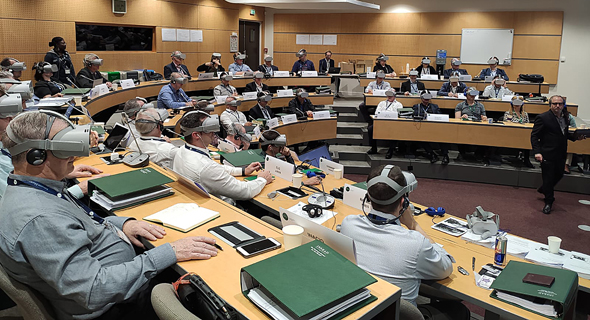
\includegraphics[scale=0.4]{img/fig2.jpg}}
\caption{Example of a figure caption.}
\label{fig}
\end{figure}

Figure Labels: Use 8 point Times New Roman for Figure labels. Use words 
rather than symbols or abbreviations when writing Figure axis labels to 
avoid confusing the reader. As an example, write the quantity 
``Magnetization'', or ``Magnetization, M'', not just ``M''. If including 
units in the label, present them within parentheses. Do not label axes only 
with units. In the example, write ``Magnetization (A/m)'' or ``Magnetization 
\{A[m(1)]\}'', not just ``A/m''. Do not label axes with a ratio of 
quantities and units. For example, write ``Temperature (K)'', not 
``Temperature/K''.

\section{Weiterbildung}

The preferred spelling of the word ``acknowledgment'' in America is without 
an ``e'' after the ``g''. Avoid the stilted expression ``one of us (R. B. 
G.) thanks $\ldots$''. Instead, try ``R. B. G. thanks$\ldots$''. Put sponsor 
acknowledgments in the unnumbered footnote on the first page.

\section{Potential}

Please number citations consecutively within brackets \cite{b1}. The 
sentence punctuation follows the bracket \cite{b2}. Refer simply to the reference 
number, as in \cite{b3}---do not use ``Ref. \cite{b3}'' or ``reference \cite{b3}'' except at 
the beginning of a sentence: ``Reference \cite{b3} was the first $\ldots$''

Number footnotes separately in superscripts. Place the actual footnote at 
the bottom of the column in which it was cited. Do not put footnotes in the 
abstract or reference list. Use letters for table footnotes.

Unless there are six authors or more give all authors' names; do not use 
``et al.''. Papers that have not been published, even if they have been 
submitted for publication, should be cited as ``unpublished'' \cite{b4}. Papers 
that have been accepted for publication should be cited as ``in press'' \cite{b5}. 
Capitalize only the first word in a paper title, except for proper nouns and 
element symbols.

For papers published in translation journals, please give the English 
citation first, followed by the original foreign-language citation \cite{b6}.

\begin{thebibliography}{00}
\bibitem{b1}  Dunleavy, M., Dede, C., and Mitchell, R. "Affordances and Limitations of Immersive Participatory Augmented Reality Simulations for Teaching and Learning". Journal of Science Education and Technology, 2009.
\bibitem{b2} H. Kaufmann, ''Collaborative Augmented Reality in Education,'' Vienna University of Technology, 
\bibitem{b3} Santos, M. E. C., Chen, A., Taketomi, T., Yamamoto, G., Miyazaki, J., and Kato, H, "Augmented Reality Learning Experiences: Survey of Prototype
Design and Evaluation". IEEE Transactions on Learning Technologies, 2014.
\bibitem{b4} A. Dengel, M. Z. Iqbal, S. Grafe and E. Mangina, ``A Review on Augmented Reality Authoring Toolkits for Education,'' Frontiers in Virtual Reality, 2022.
\bibitem{b5} H. Çetin, ``A Systematic Review of Studies on Augmented Reality Based Applications in Primary Education,'' International Journal of Education and Literacy Studies, 2022.
\bibitem{b6} M. Kesim and Y. Ozarslan, ``Augmented reality in education: current technologies and the potential for education,'' CY-ICER2012, Procedia - Social and Behavioral Sciences 47, 2012.
\bibitem{b7} H. Wu, S. W. Lee, H. Chang and J. Liang, ''Current status, opportunities and challenges of augmented reality in education,'' Elsevier, Computers and Education, 2012.
\end{thebibliography}
\vspace{12pt}

\end{document}
